\begin{figure}[bt!]
	\centering
	\subfloat[EUV image (synoptic image).]
	{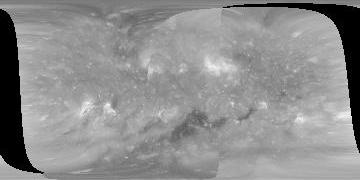
\includegraphics[width=0.47\linewidth]{pictures/thesis/chapter1/segmentation/example_syn.jpg}
		\label{subfig:Introduction_synopticImage}} 
	\subfloat[Magnetic image (photomap image).]
	{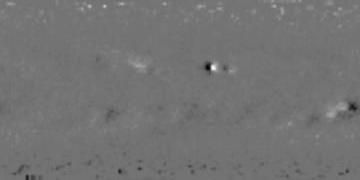
\includegraphics[width=0.47\linewidth]{pictures/thesis/chapter1/segmentation/example_photomap.jpg}
		\label{subfig:Introduction_photomapImage}} \\

	\subfloat[Model 1]{
	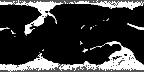
\includegraphics[width=0.33\linewidth]{pictures/thesis/chapter1/classification/m1.jpeg}
	\label{subfig:Introduction_m1}}
	\subfloat[Model 2]
	{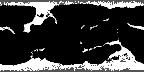
\includegraphics[width=0.33\linewidth]{pictures/thesis/chapter1/classification/m2.jpeg}
		\label{subfig:Introduction_m2}}
	\subfloat[Model 3]
	{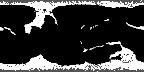
\includegraphics[width=0.33\linewidth]{pictures/thesis/chapter1/classification/m3.jpeg}
		\label{subfig:Introduction_m3}}
	        
	\subfloat[Model 4]
	{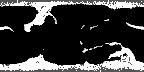
\includegraphics[width=0.33\linewidth]{pictures/thesis/chapter1/classification/m4.jpeg}
		\label{subfig:Introduction_m4}}
	\subfloat[Model 5]
	{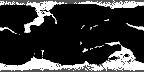
\includegraphics[width=0.33\linewidth]{pictures/thesis/chapter1/classification/m5.jpeg}
		\label{subfig:Introduction_m5}}
	\subfloat[Model 6]
	{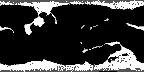
\includegraphics[width=0.33\linewidth]{pictures/thesis/chapter1/classification/m6.jpeg}
		\label{subfig:Introduction_m6}}

	\subfloat[Model 7]
	{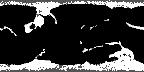
\includegraphics[width=0.33\linewidth]{pictures/thesis/chapter1/classification/m7.jpeg}
		\label{subfig:Introduction_m7}}
	\subfloat[Model 8]
	{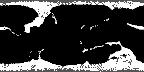
\includegraphics[width=0.33\linewidth]{pictures/thesis/chapter1/classification/m8.jpeg}
		\label{subfig:Introduction_m8}}
	\subfloat[Model 9]
	{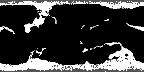
\includegraphics[width=0.33\linewidth]{pictures/thesis/chapter1/classification/m9.jpeg}
		\label{subfig:Introduction_m9}}
	
	\subfloat[Model 10]
	{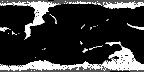
\includegraphics[width=0.33\linewidth]{pictures/thesis/chapter1/classification/m10.jpeg}
		\label{subfig:Introduction_m10}}
	\subfloat[Model 11]
	{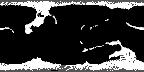
\includegraphics[width=0.33\linewidth]{pictures/thesis/chapter1/classification/m11.jpeg}
		\label{subfig:Introduction_m11}}
	\subfloat[Model 12]
	{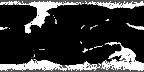
\includegraphics[width=0.33\linewidth]{pictures/thesis/chapter1/classification/m12.jpeg}
		\label{subfig:Introduction_m12}}
\caption{ 
  Physical model selection problem.
  The input images are given in (a) and (b).
  The input images need to produce coronal hole maps.
  The coronal hole maps for the physical models are shown in (c)-(n).
  Our goal is to select the physical models which produce
      the coronal hole maps that best agree with the observations.
  }
	\label{fig:Introduction_AllModels}
\end{figure}
